\documentclass[12pt,a4paper,notitlepage]{article}
\usepackage[utf8]{inputenc}
\usepackage[english]{babel}
\usepackage[T1]{fontenc}
\usepackage[backend=biber,
			style=authoryear-comp,
			isbn=false,
			doi=false,
			bibstyle=authoryear,
			natbib,
			]{biblatex}
\usepackage{eurosym}
\usepackage{enumitem}
\usepackage{url}
\usepackage{blindtext}
\usepackage{hyperref}
\usepackage{breakurl}
\usepackage{amsmath}
\usepackage{titling}
\usepackage{amsfonts}
\usepackage{amssymb}
\usepackage{pgfplots}
\usepackage{caption}
\usepackage{subcaption}
\usepackage{graphicx}
\usepackage{dcolumn}
\usepackage{tikz-3dplot}
\usepackage{subcaption}
\usepackage{float}
\usepackage{adjustbox}
\usepackage{multirow,rotating}
\usepackage[autostyle]{csquotes}
\usepackage[toc,page]{appendix}
\usepackage{lscape}
\usepackage{todonotes}
\usepackage{booktabs}
\usepackage{multirow}
\usepackage{bm}
\usepackage{eurosym}

\addbibresource{Textmining.bib}

\begin{document}

\section{Introduction}

Social networks such as Facebook are becoming more and more important for online news services: an increasing number of their readers access the news pages via links in the networks. Users of Facebook, for example, can use their profile to share links to external websites - such as news portals - with their online friends. This has led to the development of social media becoming an important generator of traffic for content providers. In Germany, 94\% of online shared news articles in 2015 are distributed via Facebook, followed by Twitter with 3.5\% and Google+ with 2.3\% \citep{schiller_development_2016}. 

The advertising-financed business model of the media houses is based on the premise that users visit their websites in order to achieve high advertising revenues. For this reason, news agencies are particularly interested in finding out which topics are more likely shared on these platforms. \citet{schiller_development_2016} show, that social media users choose a certain site depending on the researched topic. FOCUS Online for example is targeted for articles from politics and business, while sports news is more likely to be shared from Bild.de. 

While these pre-defined resorts give an indication on the content of an article, multiple articles in the same resort probably don't cover the same topics. Especially if the articles originate from different news portals. Furthermore, articles can contain more than one topic. We use a structural topic model to reveal the underlying topics of a collection of articles, and how the articles exhibit them. We then estimate the effect of topic prevalence on the number of Facebook shares. 

Mapping raw text to one or more topics, without having prior knowledge on what those topics are, translates to an unsupervised classification problem on natural language. Topic models generate low-dimensional representations of data and can uncover interesting latent structure in large text datasets. They are popular tools for automatically identifying prominent themes in text. Within topic models the Latent Dirichlet Allocation (LDA) is a widely used technique, where each document (article) is viewed as a mixture of topics (represented by the document-topic distribution) and each topic is a mixture of unique terms, represented by the topic-term distribution \citep{blei_latent_2003}. \citet{roberts_model_2016} extents the base idea of LDA by developing a structural topic model (STM) that allows to incorporate external variables that effect both topical content and topical prevalence. We use this approach to analyze online news about the german federal elections, where we allow prevalence of topics to vary across newswire services. We then estimate the effect of topical prevalence (the posterior document-topic distribution) on the number of Facebook shares.

Figure \ref{fig_research_strat} gives an overview of the applied research strategy. Chapter \ref{ch_model} explains the generative process of the mixed membership model and the results of this process are presented in chapter \ref{ch_results}. Chapter \ref{ch_data} contains a description of the text data and how it was pre-processed in order to use it as input variable.  Chapter \ref{ch_regression} describes how we regress the estimated probabilities of topic prevalence of a document on the times, this document was shared on Facebook.

\begin{figure}[ht]
	\centering
	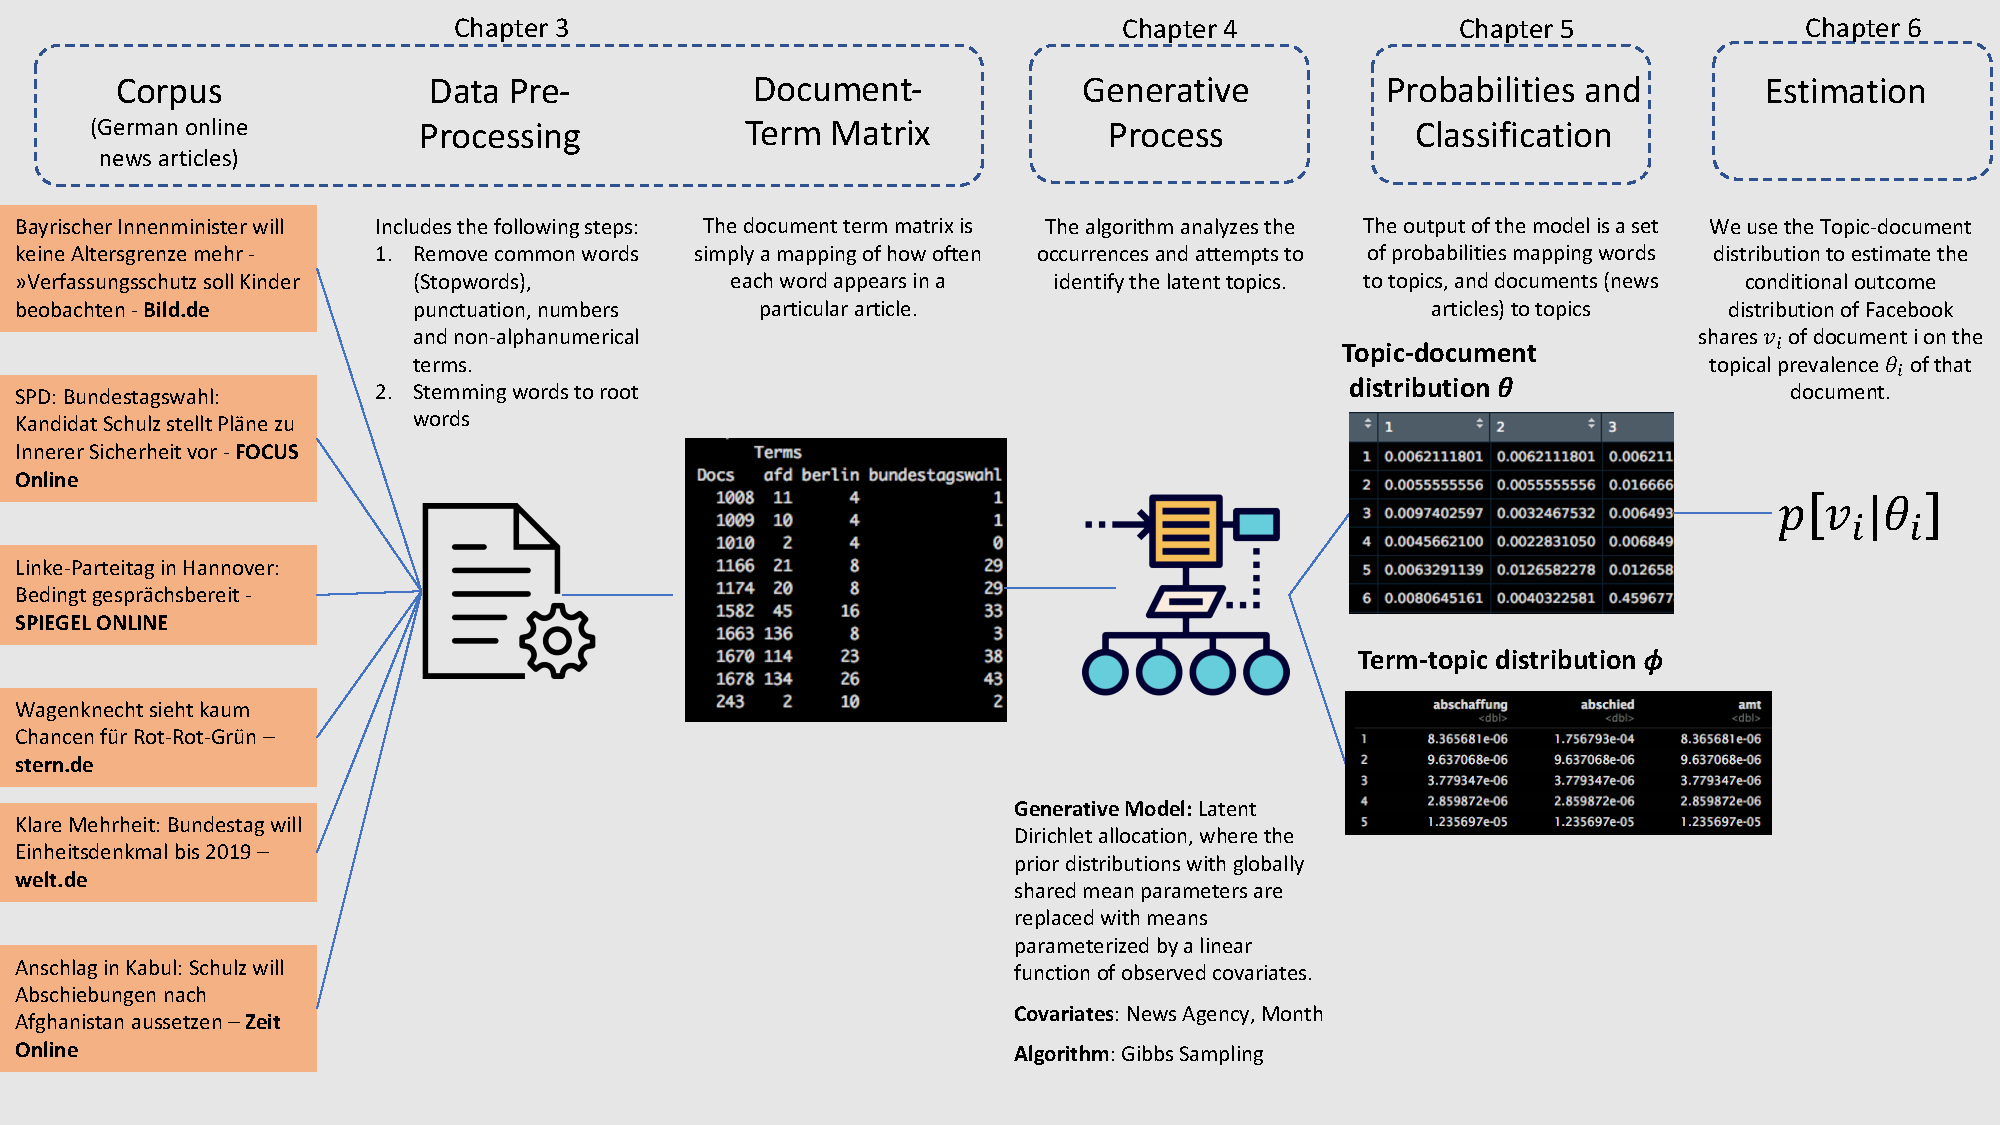
\includegraphics[width=0.95\textwidth]{../figs/research_strategy.pdf} 
	\caption{Research Strategy}
	\label{fig_research_strat}
\end{figure}

% Related Literature
% ------------------
\section{Related Literature}
% ---------------------------------------
% Business Model in the online news market
% --------------------------------------- 
\subsection{The online news market}

Media outlets naturally appear as two-sided platforms, that allow interaction between two categories of consumers: audiences and advertisers. The demand on both consumer-sides are often linked via indirect network externalities. The market in which media outlets operate are accordingly referred to as two-sided or multi-sided markets. The theoretical literature on two-sided markets originates from the analysis of credit card markets \citep{rochet_platform_2003} and was later transferred to the concept of other industries, such as dating agencies, real estate agents, and internet “business-to-business” websites \citep{caillaud_chicken_2003}. The basic concept of two-sided markets was already discussed decades ago in several economic studies, especially on media markets \citep{corden_maximisation_1952}, \citep{gustafsson_circulation_1978}, \citep{blair_pricing_1993}. However, comprehensive analyses have only been carried out in the last ten years, starting with the works of \citet{rochet_platform_2003}, \citet{evans_empirical_2003} and \citet{armstrong_competition_2006}.

Online news are typical examples of two-sided markets where the news pages can be conceived as platforms that allow interaction between audiences ("eyeballs") and advertisers. The size and characteristics of the audience has a positive effect on the advertisers' willingness to pay, as advertisements are typically sold based on cost per viewer, often expressed in terms of the cost of reaching a thousand viewers (CPM). Advertising can also have an effect on the recipients, which can be both negative and positive, depending on the quality of the advertising. 

Depending on the strength of the indirect network effects, publisher maximize their revenue by balancing the demand from advertisers and subscribers using different business models \citep{evans_economics_2008}. Many traditional newspapers follow the subscription/advertising model, where the publisher charges both market sides: The audience pays a fee to obtain access to the content, and advertisers pay to to obtain access to the viewers. Many online news agencies also provide a part of their editorial content as a premium service. However, since the Internet has considerably simplified the possibilities for obtaining information and thus reduced the marginal utility of content, such a business model can only function if the content is very exclusive. As a result, many publishers rely on a free-media model, in which the publishers do not charge viewers for access to the media at all, in order to attract as many readers as possible to their platform, and thus exploit the indirect network effects on the advertising site. % What is the share of advertising revenue in total earnings of german online newspaper ? 

In addition to the quantity of the audience, the demographic characteristics of recipients also have an influence on the willingness to pay on the advertiser site. Online advertising makes it possible to target ads to particular consumers in real time. Facebook instant articles facilitates this targeting, as they make the public users profile data available to the publisher. 

The two-sided market structure of news markets results in news platforms striving to choose their content in such a way that its reach is as large as possible in order to maximize profits from advertising revenues. This may lead to media-bias, as advertising may affect the ability and incentives of media to provide independent news. On the other hand, advertising may also have a positive impact on the media, as it enables publishers to report independently of political parties. \citet{ellman_what_2009} found that advertising increases the intensity of competition for readers and therefore raises accuracy of media coverage.  

% --------------
% Topic Modeling
% --------------
\subsection{Topic Modeling}

We use the structural topic model (STM) developed by \citet{roberts_model_2016} that allows us to incorporate document specific covariates (e.g. the author or date of a document). STM is a recent extension of the standard topic modeling technique, labeled as "latent Dirichlet allocation" (LDA), which refers to the Bayesian model in \citet{blei_latent_2003} that treats each word in a topic and each topic in a document as generated from a Dirichlet - distributed prior.\footnote{See also \citet{griffiths_probabilistic_2002}, \citet{griffiths_finding_2004} and \citet{hofmann_probabilistic_1999}. \citet{pritchard_inference_2000} introduced the same model in genetics for factorizing gene expression as a function of latent populations.} Topic models formalize the idea that documents are formed by hidden variables (topics) that generate correlations among observed terms. Since its introduction into text analysis, LDA has become hugely popular and especially useful in political science.\footnote{see \citet{blei_probabilistic_2012} and \citet{grimmer_text_2013} for an overview.}

The basic topic model has been extended in variety of ways. \citet{blei_dynamic_2006} considers documents that are indexed by publication date date and allows the topics to evolve in time. To relax the assumption that all texts in the modeled corpus are generated by the same underlying process, \cite{roberts_model_2016} introduces the structural topic model (STM), that provides a way to include covariates. Using a generalized linear model on document-level metadata allows the researcher to link topics to covariate data and to model changes in topic prevalence over time. 

STM has been applied to multiple academic fields: \citet{roberts_structural_2014} uses STM to analyse open-ended responses from surveys and experiments, \citet{farrell_corporate_2016} applies the model to scientific texts on climate change, revealing links between corporate funding and the framing of scientific studies and \citet{mishler_using_2015} shows that "STM can be used to detect significant events such as the downing of Malaysia Air Flight 17" when applied to twitter data. Another study shows how STM can be used to explore the main international development topics of countries’ annual statements in the UN General Debate and examine the country-specific drivers of international development rhetoric \citep{baturo_what_2017}. \citet{mueller_reading_2016} uses newspaper text to predict armed conflicts in different regions. They use the estimated topic shares in linear fixed effects regression to forecast conflict out-of-sample.

% -----
% Data
% -----
\section{Dataset}\label{ch_data}

We conduct our estimation on a sample of 10531 news articles containing the term "Bundestagswahl" (Federal Election) dated from 01.06.2017 to 28.10.2017.\footnote{German federal elections took place on 24th of September 2017.} We first extract all online articles of six mainstream german online news portals\footnote{Bild.de, Focus.de, Spiegel.de, Stern.de, Welt.de, Zeit.de} using the the Event Regestry API.\footnote{For more information see http://eventregistry.org/documentation. The scraping code was written in Python and can be made available on request.} We then filter those articles that contain the term "Bundestagswahl" (Federal Election) in their text body. We use the URL of these articles, to check how many times they where shared on Facebook using the \textit{sharedcount} API.\footnote{http://docs.sharedcount.com/} The returned share count is the sum of (1) the number of likes of this URL, (2) the number of shares of this URL (including copy-pasting a link back to Facebook), (3) the number of likes and comments on stories on Facebook about this URL and (4) the number of inbox messages containing this URL as an attachment.\footnote{See https://developers.facebook.com/docs/graph-api for more information about the Facebook Graph API.}

Figure \ref{fig_distr1} shows the distribution of the number of articles from the respective news sources by date. There is a high peak around the federal elections on September, 24th. Most of the articles are published by welt.de, followed by stern.de (see \ref{fig_distr2}).  

\begin{figure}[H]
	\caption{Article distribution...}
	\begin{center}
		\begin{subfigure}[normla]{0.49\textwidth}
			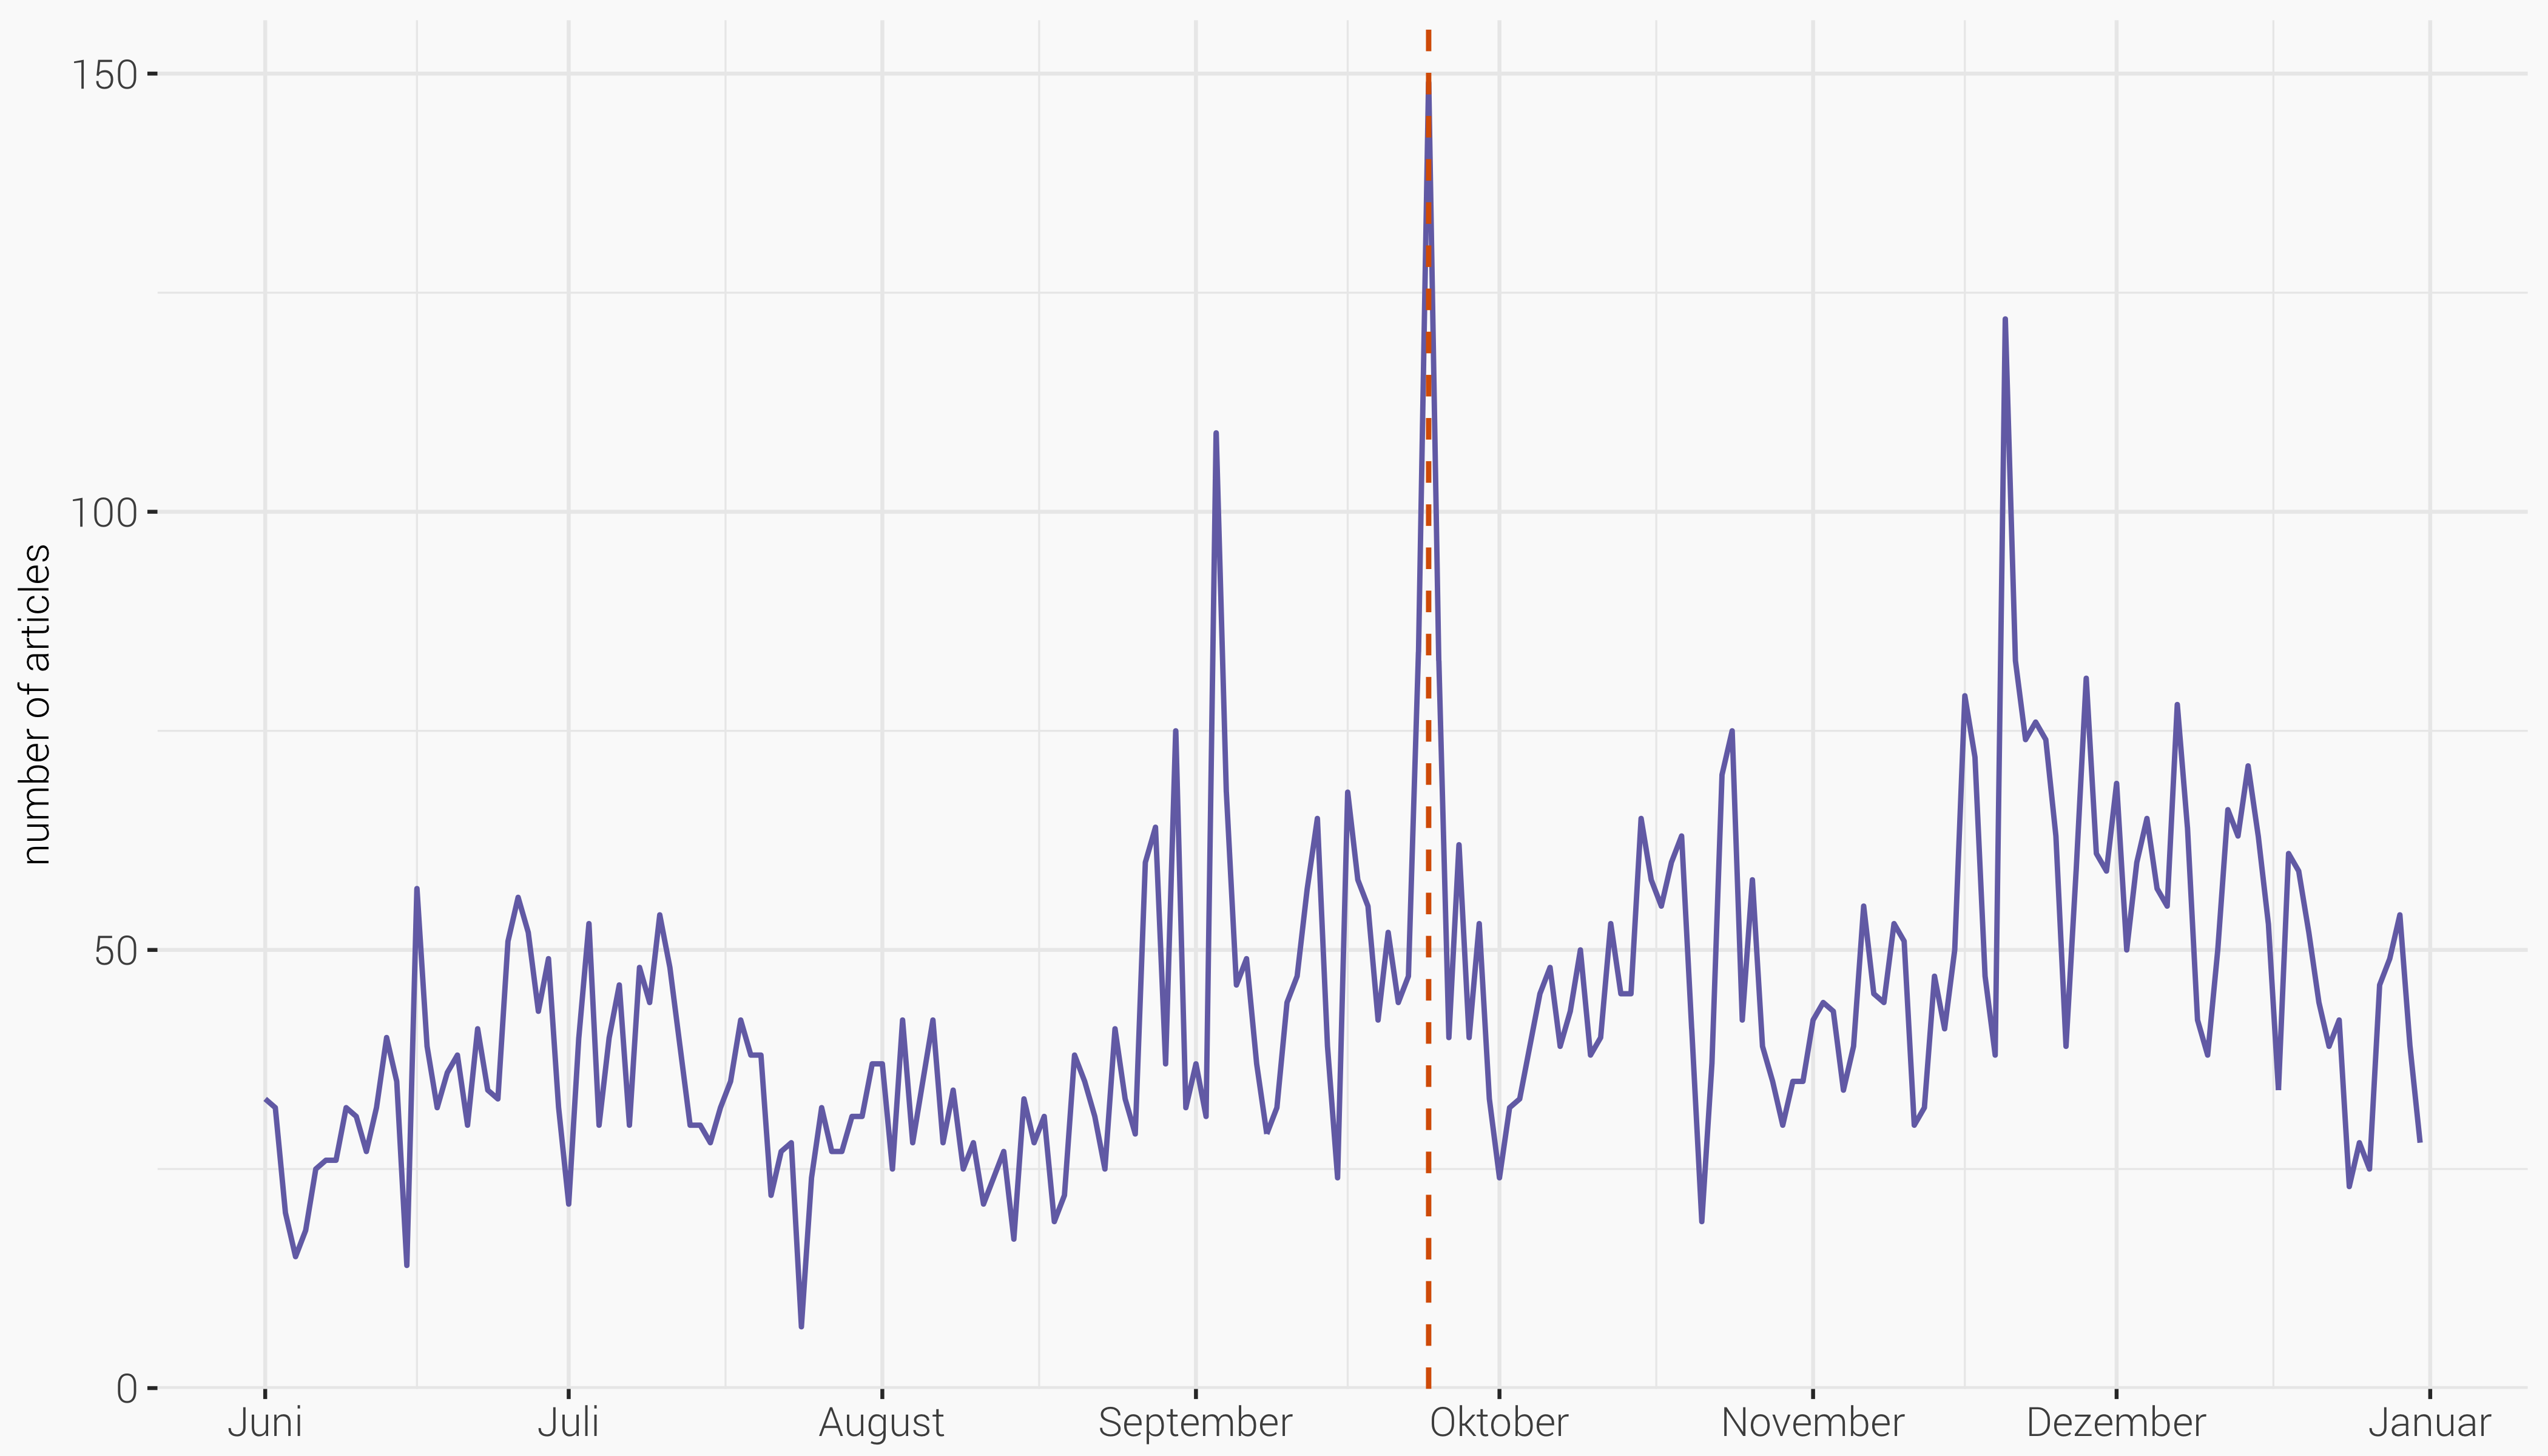
\includegraphics[width=\textwidth]{../figs/timeline.png}
			\caption{...by date \& news source}
			\label{fig_distr1}
		\end{subfigure}
		\begin{subfigure}[normla]{0.49\textwidth}
			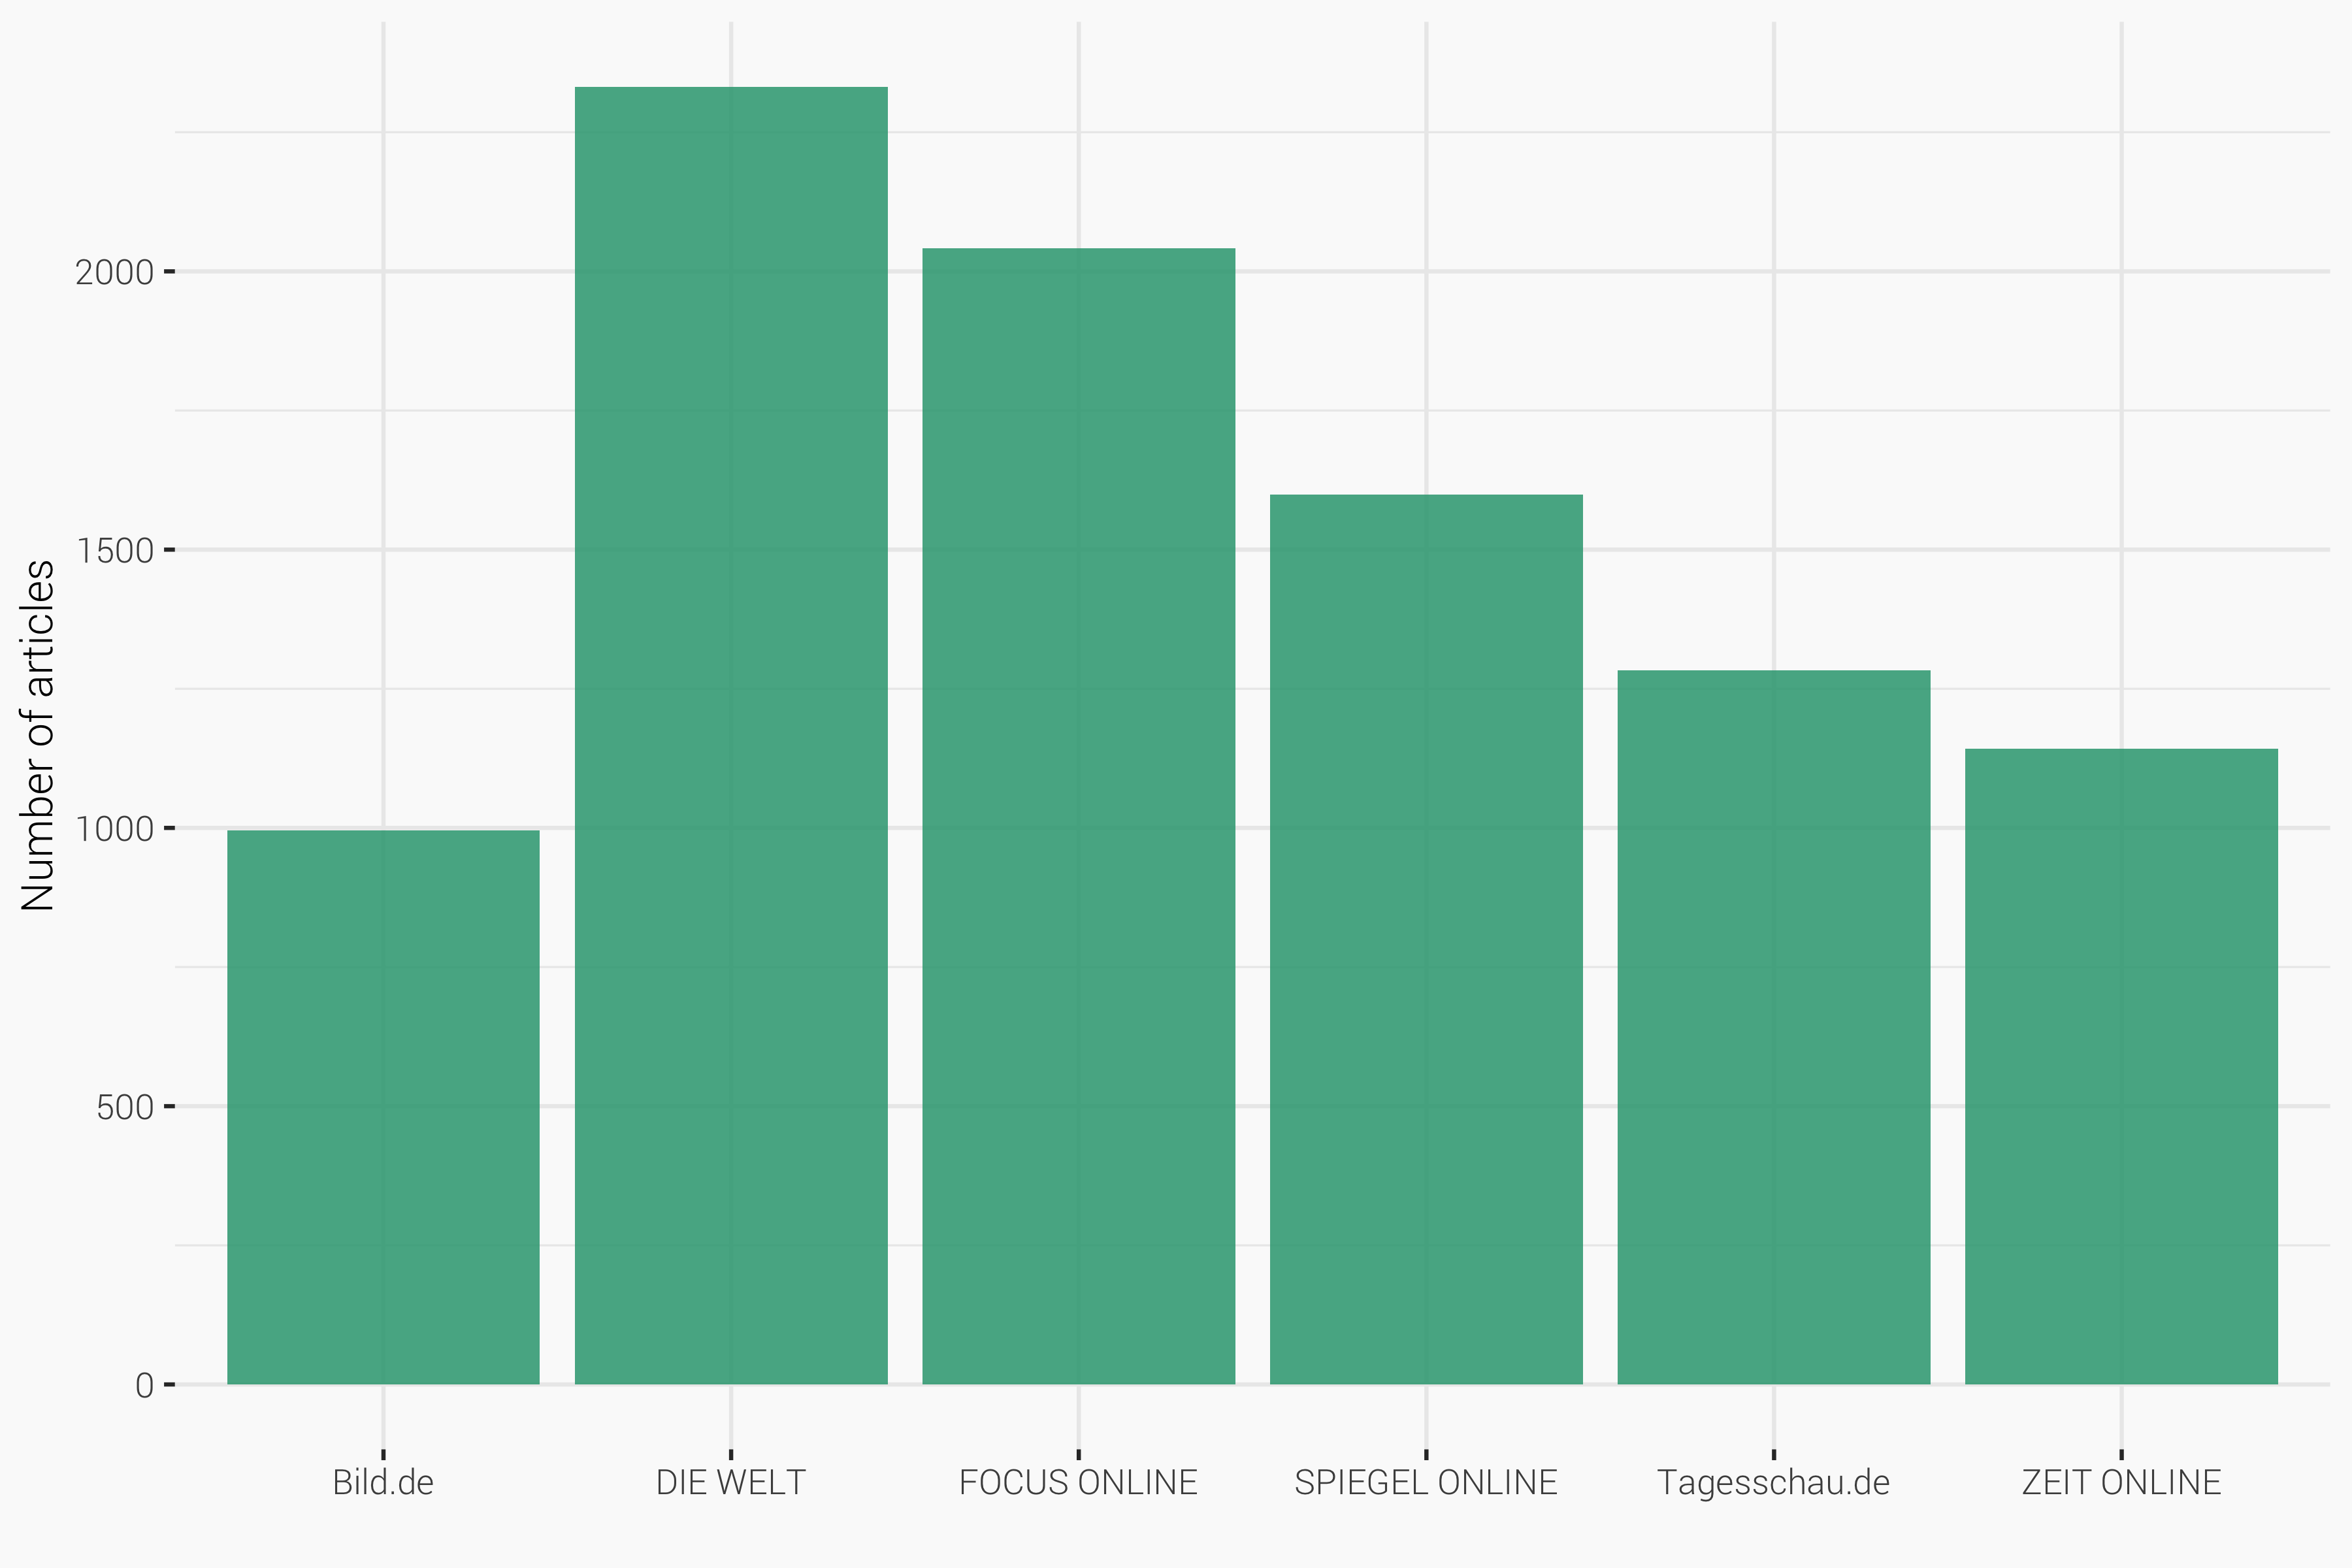
\includegraphics[width=\textwidth]{../figs/bar.png}
			\caption{... by news source}
			\label{fig_distr2}
		\end{subfigure}
	\end{center}
\end{figure}

\begin{figure}[H]
	\caption{Distribution of Facebook shares...}
	\begin{center}
		\begin{subfigure}[normla]{0.49\textwidth}
			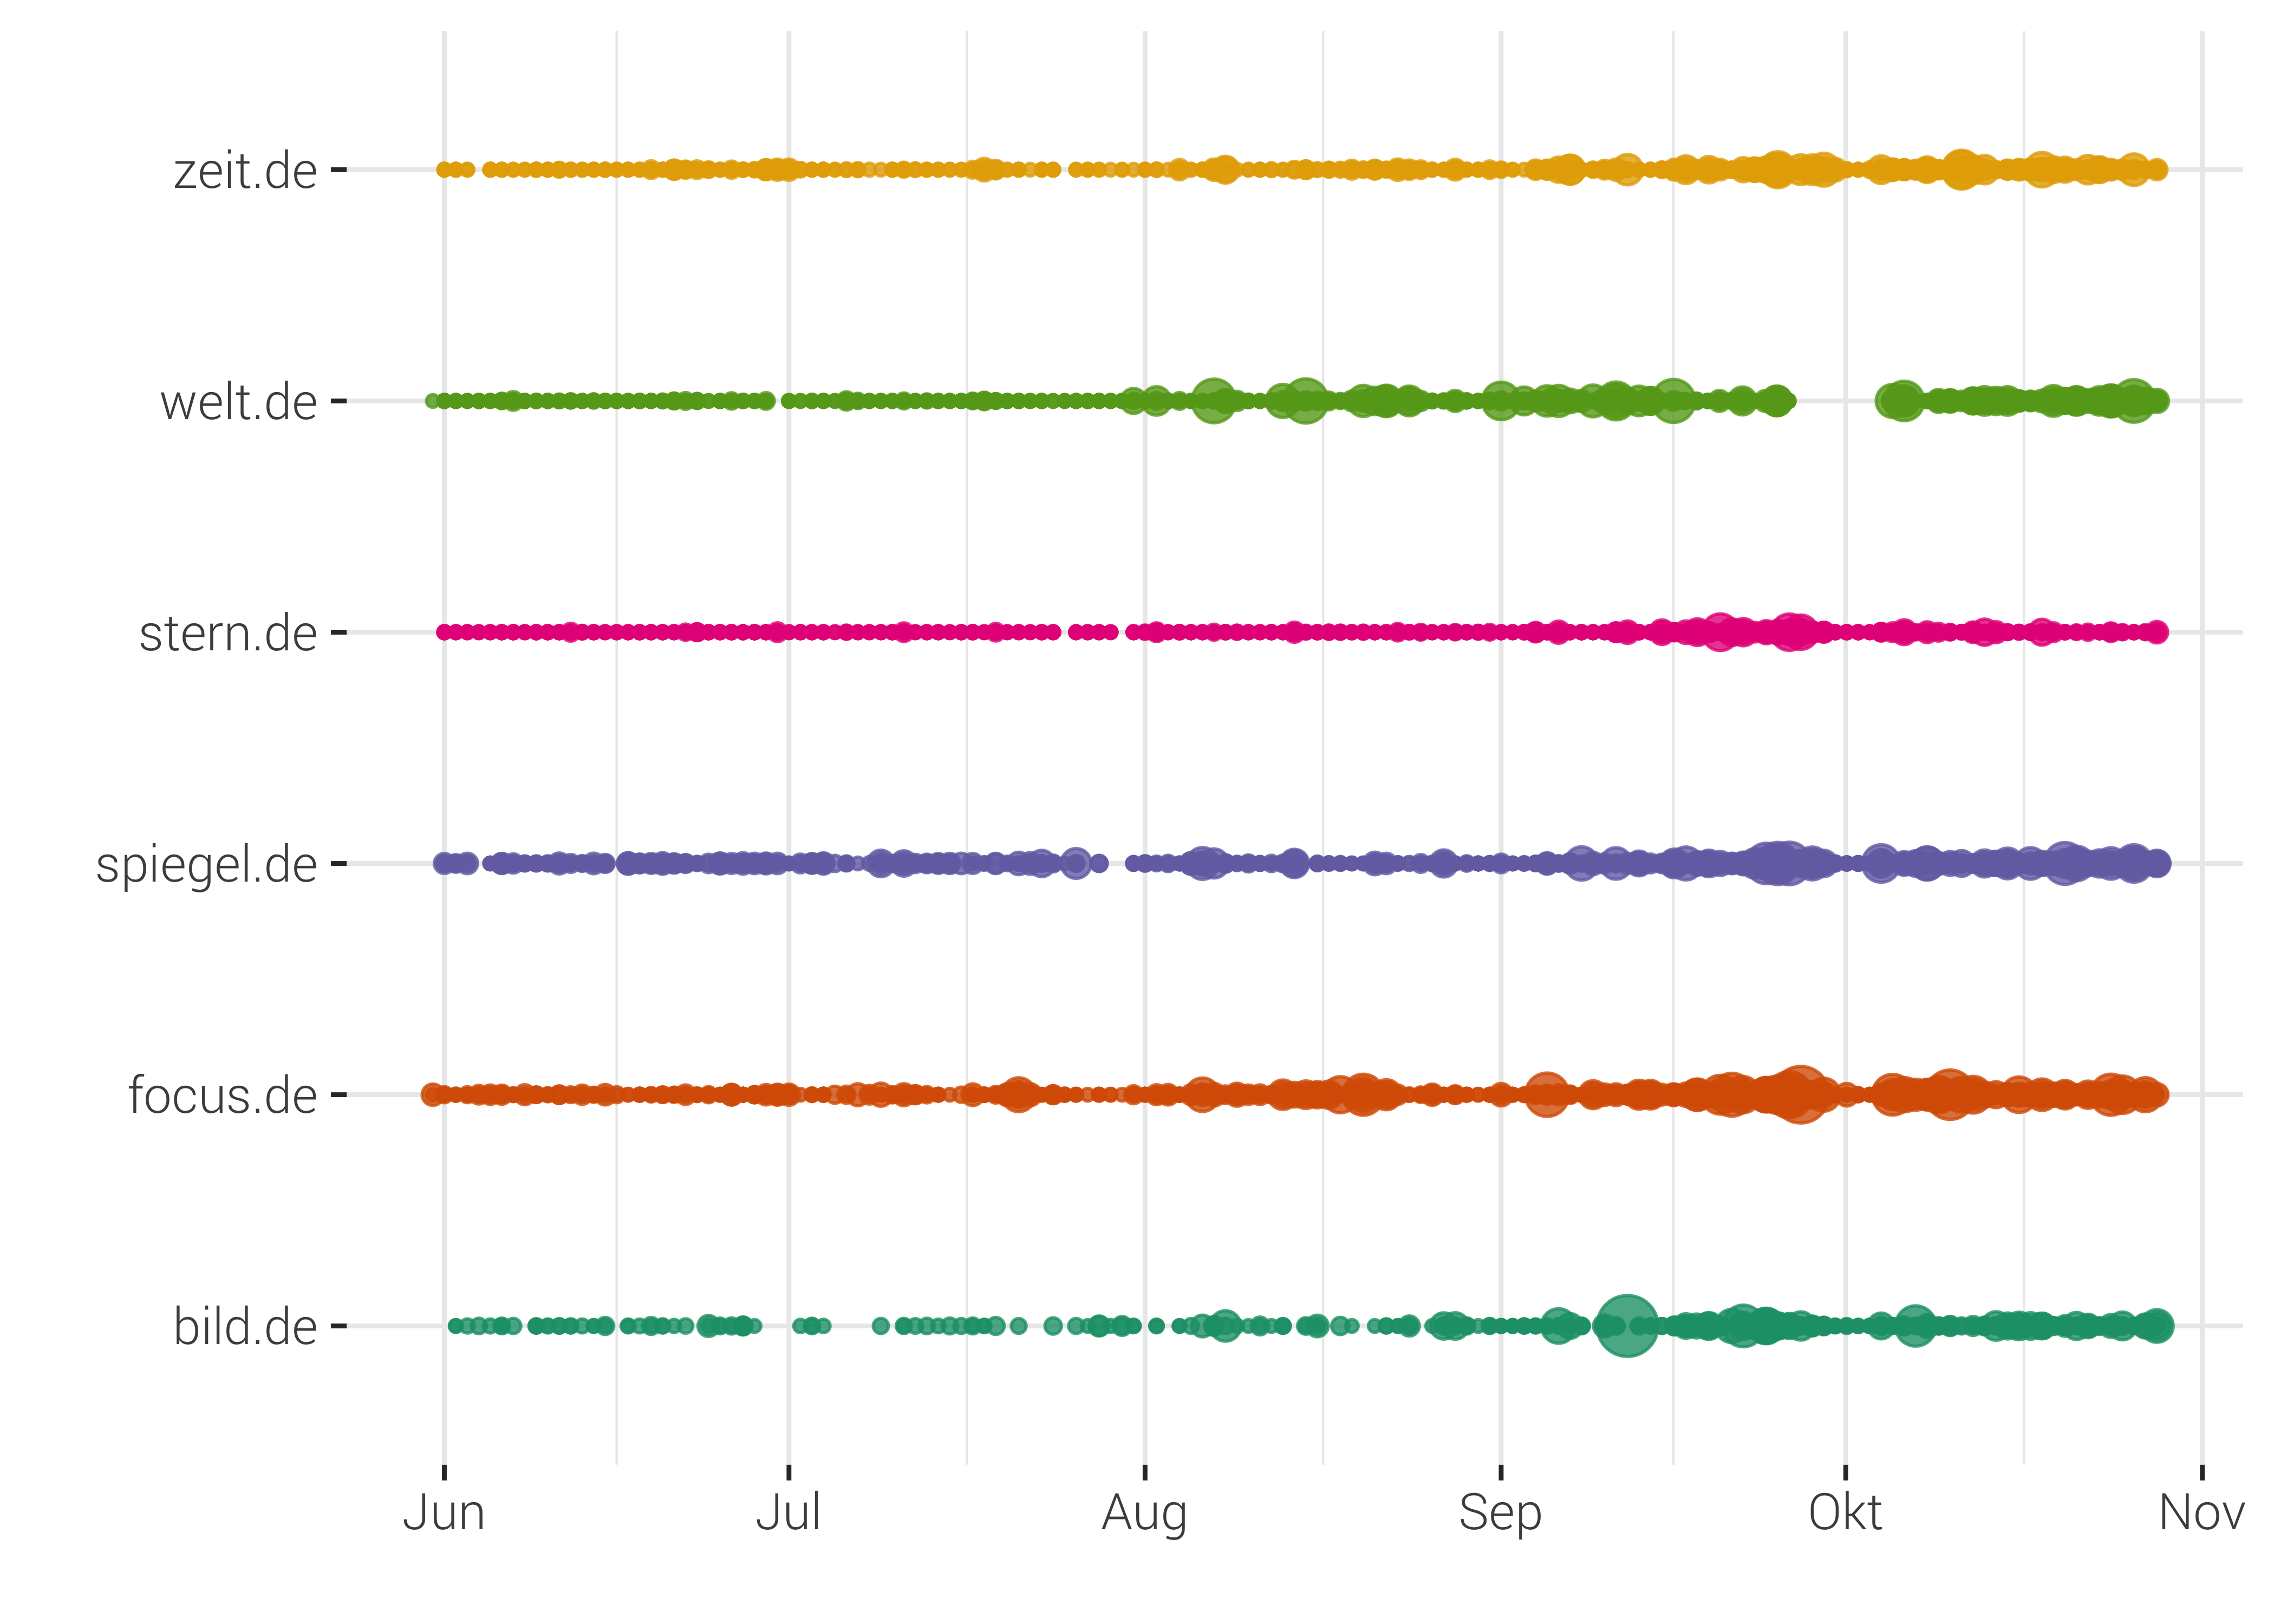
\includegraphics[width=\textwidth]{../figs/fb_shares.png}
			\caption{...by date \& news source}
		\end{subfigure}
		\begin{subfigure}[normla]{0.49\textwidth}
			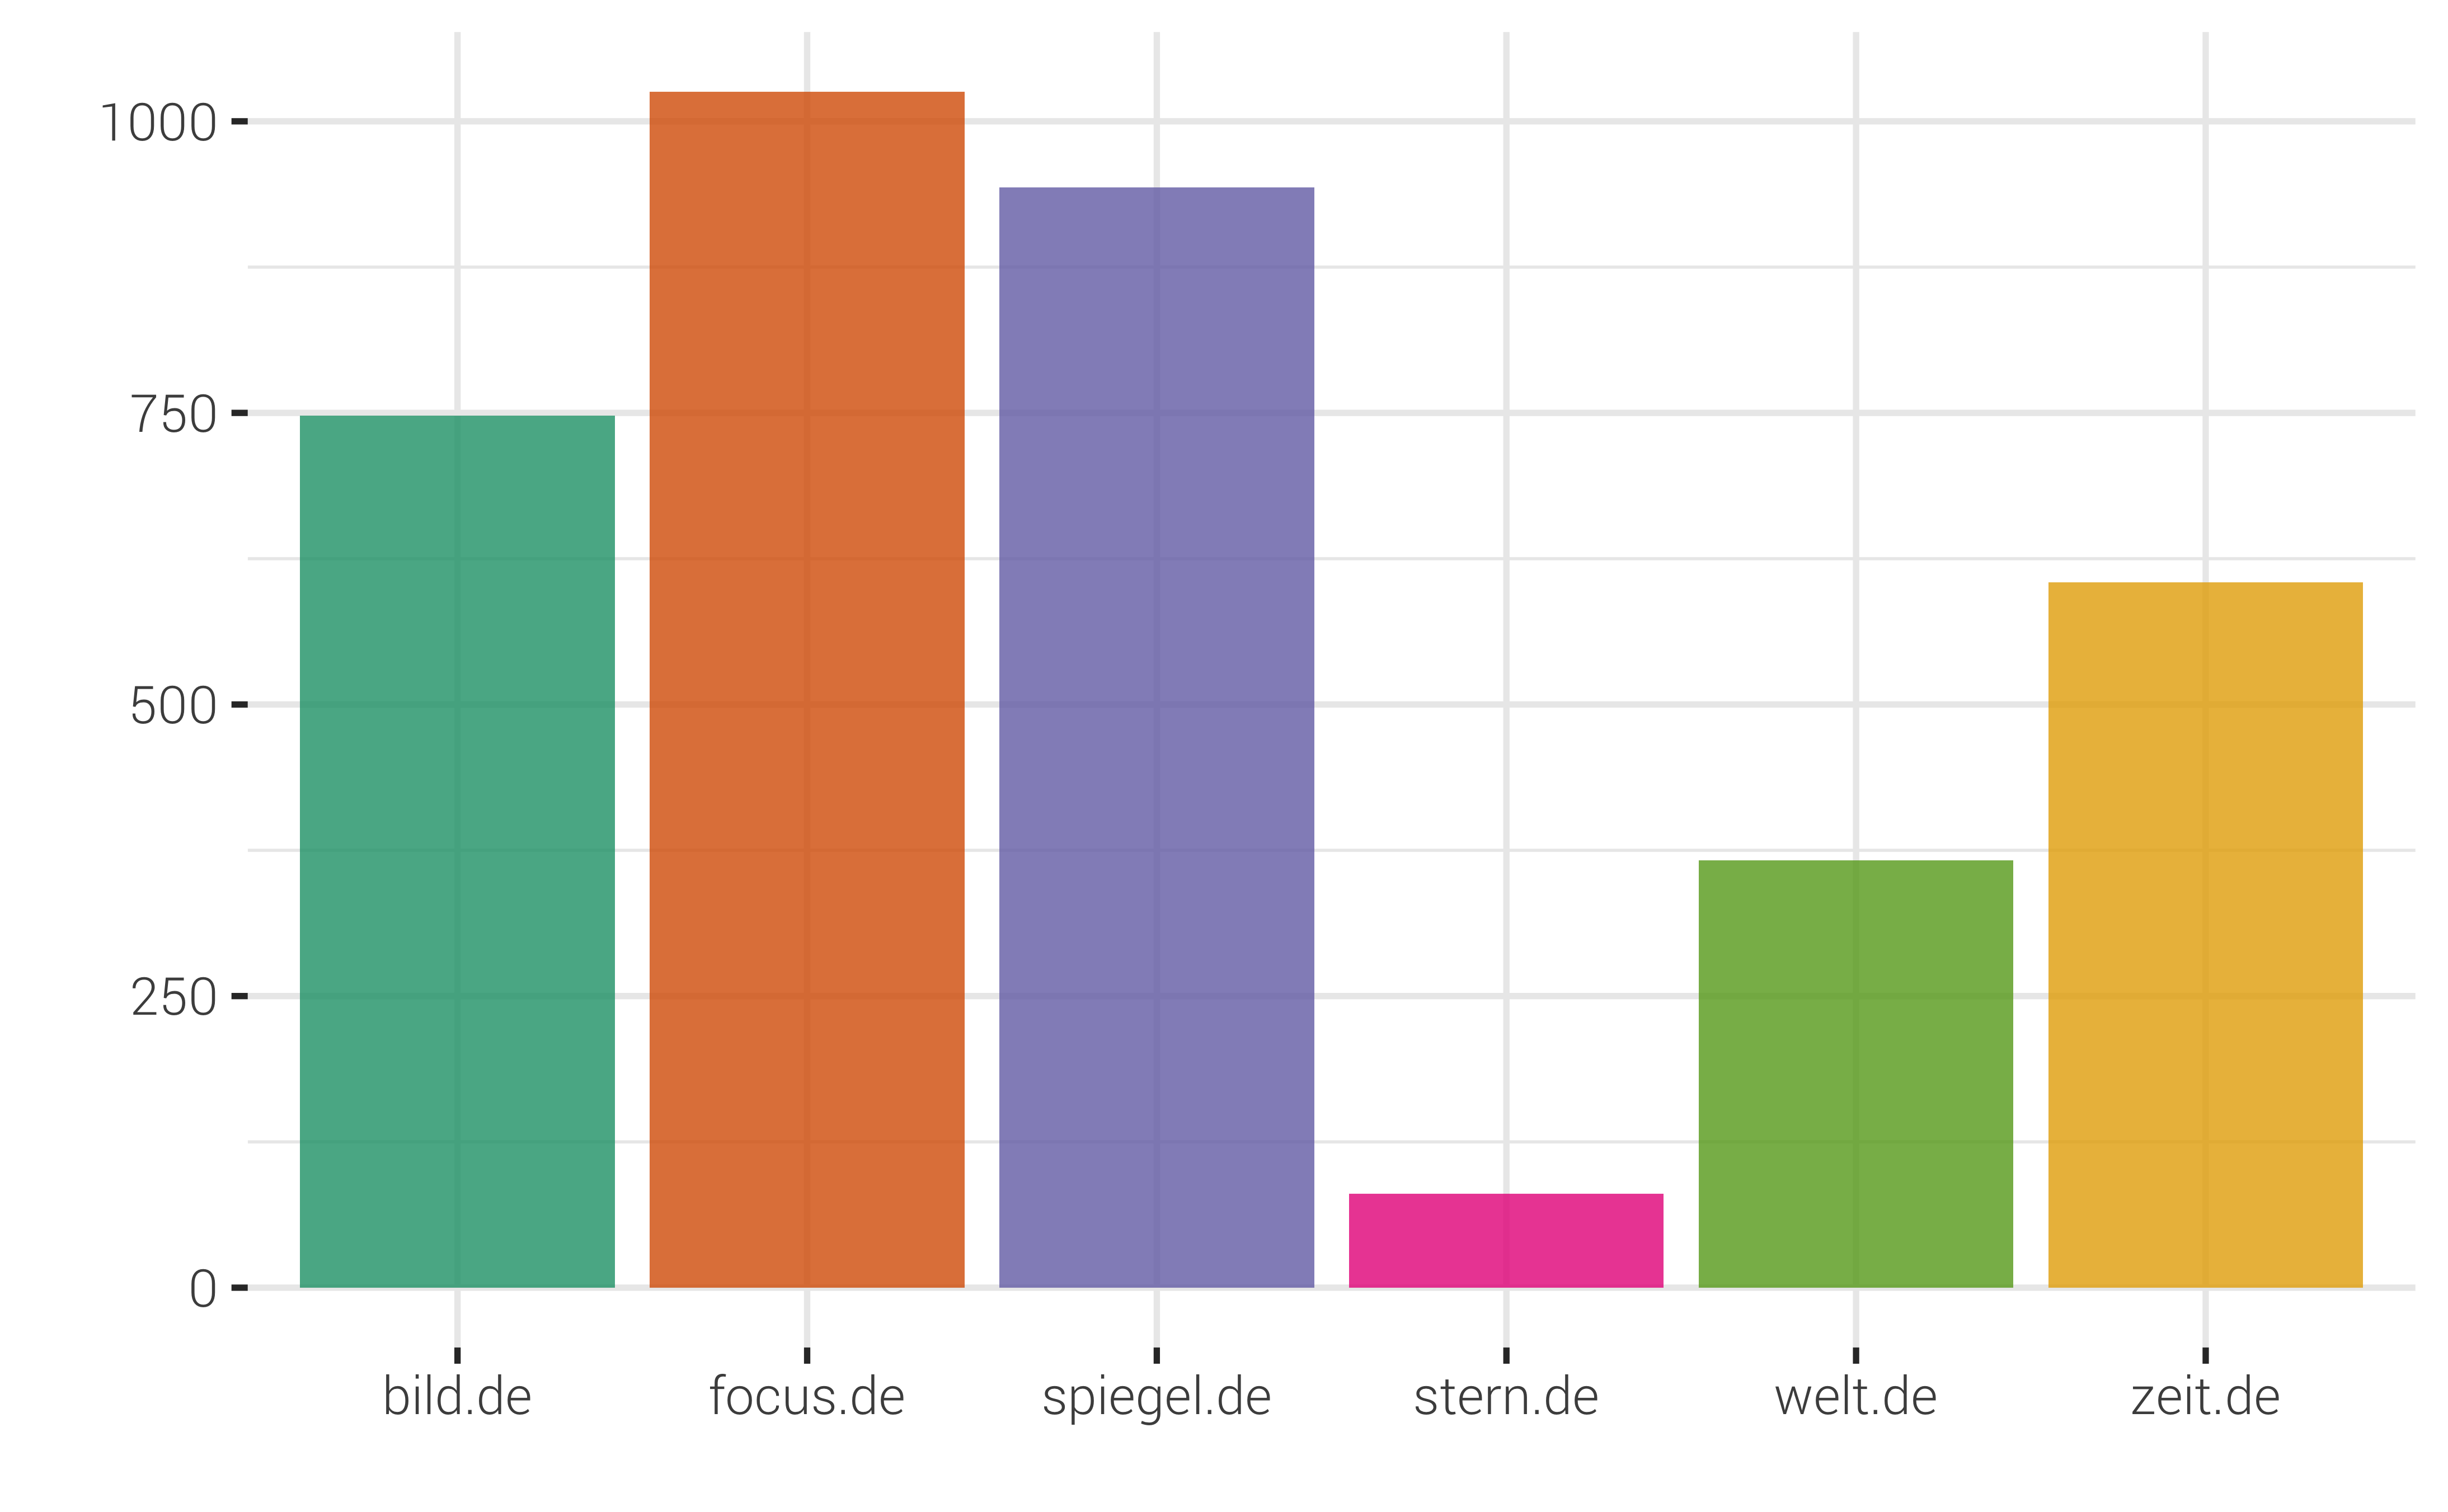
\includegraphics[width=\textwidth]{../figs/fb_shares_mean.png}
			\caption{... by news source (mean)}
		\end{subfigure}
	\end{center}
	\label{fig_fb_shares}
\end{figure}

To use text as data and reduce the dimensionality, a common strategy is to pre-process the text by imposing some preliminary restrictions (stop-word removal, tokenization) based on the nature of the data (twitter text, newspaper articles, speeches, etc.) to reduce the number of language elements to consider \citep{gentzkow_text_2017}. An overview of how these steps were applied to our data set can be found in the next section. 

After pre-processing, each document $d$ is a finite list of terms. Each unique term in the corpus is indexed by some $v \in \lbrace 1,...,V \rbrace$ where $V$ is the number of unique terms. For each document $d \in \lbrace 1,...,D \rbrace$ we compute the number of occurrences of term $v$ in document $d$ to obtain the count $x_{d,v}$. The $D$ x $V$ matrix $\boldsymbol{X}$ of all such counts is called the document-term matrix. This representation is often referred to as the bag of words model, since the order in which words are used within a document is completely disregarded. 


% ------------------
% Text Pre-Procesing
% ------------------
\subsection{Text pre-procesing}

A central task in text mining is to extract low-dimensional information from documents that are high-dimensional by nature \citep{bholat_text_2015}. This is related to the task of reducing the number of unique language elements in order to reduce the dimensionality of data (to avoid unnecessary computational complexity and overfitting) while at the same time keeping those words that reflect the content of a document. Any useful representation of text will throw away some information, the trick is to include the relevant information for our needs, and exclude the extraneous information. 

Intuitively the term frequency (tf) of a word is a measure of how important that word may be. There are words in a document, however, that occur many times but may not be important like articles, conjunctions, and so on. These terms, often called "stop words", are important to the grammatical structure of a text, but typically don't add any additional meaning and can therefore be neglected. We use a pre-defined stop word list from the Snowball stemmer project\footnote{http://svn.tartarus.org/snowball/trunk/website/algorithms/*/stop.txt} together with a customized list of stop-words that are redundant superfluous or distorting. We also remove punctuation character (e.g. ., ,, !, ?, etc.) and all numbers from our corpus.  

% ----------------------
% Structural topic Model
% ----------------------
\section{Topic detection}\label{ch_model}

The following description of the generative model of the STM is based on \citet{roberts_structural_2013} and \citept{roberts_stm:_2016}. The process of filling a word-position in a document begins with the generation of a document-specific topic-prevalence vector $d(\boldsymbol{\theta}_d)$ drawn from a logistic-normal distribution, where the parameters are a function of the covariate values:

\begin{align*}
	\boldsymbol{\theta}_d|\boldsymbol{x}_{d\gamma},\boldsymbol{\Sigma} \sim \textrm{LogisticNormal}(\mu = \boldsymbol{x}_{d\gamma}\boldsymbol{\Sigma})
\end{align*}

$\boldsymbol{x}_d\gamma$ lists the values of all metadata covariates for document $d$, where $\gamma$ relates these covariate values to the topic-prevalence. The structure of $\boldsymbol{\Sigma}$ implies the possibility of correlations across documents in the topic-prevalence vector which help enhance interpretation and prevent overfitting. 

Given the document-specific distribution over topics, for each word in the document ($n \in \lbrace 1,...,N_d\rbrace$) is assigned to a specific topic $z_{dn}$ through the process

\begin{align*}
	z_{dn}|\boldsymbol{\theta}_d \sim \textrm{Multinomial}(\boldsymbol{\theta}_d)
\end{align*}

where the $k^{th}$ element if $z_{dn}$ is unity and all other elements are zero when topic $k$ is chosen. 

Conditional in the topic chosen, a specific word, $w_{dn}$, is chosen from the overall corpus vocabulary $V$ to fill position $n$ in document $d$, using the following process:

\begin{align*}
	w_{dn}|z_{dn},\beta_{dkv} \sim \textrm{Multinomial}(\beta_{dk1},...,\beta_{dkV}).
\end{align*}

where the word probability $\beta_{dkv}$ is modeled as a function of the two parameters $m_v$ (indicating the importance of that word across all documents) and $\kappa_{kv}$ (indicating the importance of the word given the topic $k$). Transforming the sum of these coefficients into probabilities for use in a multinomial distribution via logistic transformation, one obtains:

\begin{align*}
	\beta_{dkv}|z_{dn}\propto\textrm{exp}(\boldsymbol{m}_v+\kappa_{kv})
\end{align*}


The STM maximizes the posterior likelihood that the observed data were generated by the above data-generating process using an iterative approximation-based variational expectation-maximization algorithm available in R's stm package \citep{roberts_stm:_2016}. Regularizing prior distributions are used for $\gamma$, $\kappa$ and (optionally) $\Sigma$. To address problems due to non-convexity, we rely on the spectral initialization approach advocated by \citet{roberts_navigating_2016}.

% ----------------------
% Model Selection
% ----------------------
\subsection{Model selection}

Topic models are generally inaccurate, since the number of topics must be determined a priori. Furthermore, multiple solutions exist for the optimization problem. Ex post analysis of several model specifications helps to evaluate its quality, as well as the number of topics and metadata selected. 

The most common choice is the probability of held-out documents \citep{grimmer_bayesian_2010}. Similar to cross-validation (VC), different model specifications are compared to how well they do in predicting words within a document \citep{asuncion_smoothing_2012}, \citep{wallach_evaluation_2009}. Another strategy to find an appropriate number of topics is to check for residual overdispersion of the variance of the multinomial within the data generating process of the model \citep{taddy_estimation_2012}. Other approaches can be found in \citet{airoldi_reconceptualizing_2010} and \citet{teh_hierarchical_2006}. We run multiple model specifications and compare them based on held-out likelihood estimation, residual checks as well as semantic coherence to chose the number of topics that best fits the corpus to be 50. Furthermore, we use the source of each article (the media house) and the month it was published as a covariates in the topic prevalence portion of the model. In other words, the probability distribution of topics depends on the editorial strategy of a media house as well as on the month the article was published. 

% ----------------------
% Evaluation
% ----------------------
\subsection{Evaluation}


The most effective method for assessing model fit is to carefully read documents that are closely associated with particular topics to verify that the semantic concept covered by the topic is reflected in the text. The parameter θd provides an estimate of each document’s association with every topicmaking it straightforward to effectively direct analyst engagement with the texts (see, e.g., Roberts, Stewart, and Tingley 2014a). An overview of manual validation procedures can be found in Grimmer and Stewart (2013).\cite{roberts_model_2016}

To validate the accuracy with which the fitted model is capturing the content of a document, we first conduct a process of informal manual audits \citep{gentzkow_text_2017}: We inspect inspect a subset of documents alongside the fitted topics to cross-check against the coding a human would produce by hand. Figure \ref{fig_classification} shows sample documents classified to each topic for reference. We produce a random sample of 7 posts from the 300 highest probability fits per topic.

\begin{figure}[H]
\centering
	\caption{Sample articles}
	\includegraphics[width=\textwidth]{../figs/topic-classification-sample.png}	
	\label{fig_classification}
\end{figure}

The interpretability or semantic coherence of topics can vary considerably. \citet{mimno_optimizing_2011} propose a topic semantic coherence score computed from in-corpus word co-occurrence statistics, and show strong agreement with human evaluations. 

\cite{mimno_optimizing_2011}
The evaluation of statistical topic models has traditionally been dominated by either extrinsic methods (i.e., using the inferred topics to perform some external task such as information retrieval \citep{wei_lda-based_2006} or quantitative intrinsic methods, such as computing the probability of held-out documents \citep{wallach_evaluation_2009}. Recent work has focused on evaluation of topics as semantically coherent concepts. For example, \citet{chang_reading_2009} found that the probability of held-out documents is not always a good predictor of human judgments.


After performing the topic modeling, we can generate an overview of the news landscape about the german elections. Each group is composed of the most relevant words for that topic, and a manually-determined label. The distances that the topics have from each other reflect their semantic distance, or basically how different the words are for that topic. It is computed as the Jensen-Shannon divergence between each of the topics according to the differences in their word-topic probabilities. We then apply principal coordinates analysis in order to project the distance matrix down to two dimensions.

%\begin{figure}[H]
%\centering
%	\caption{News Landscape}
%	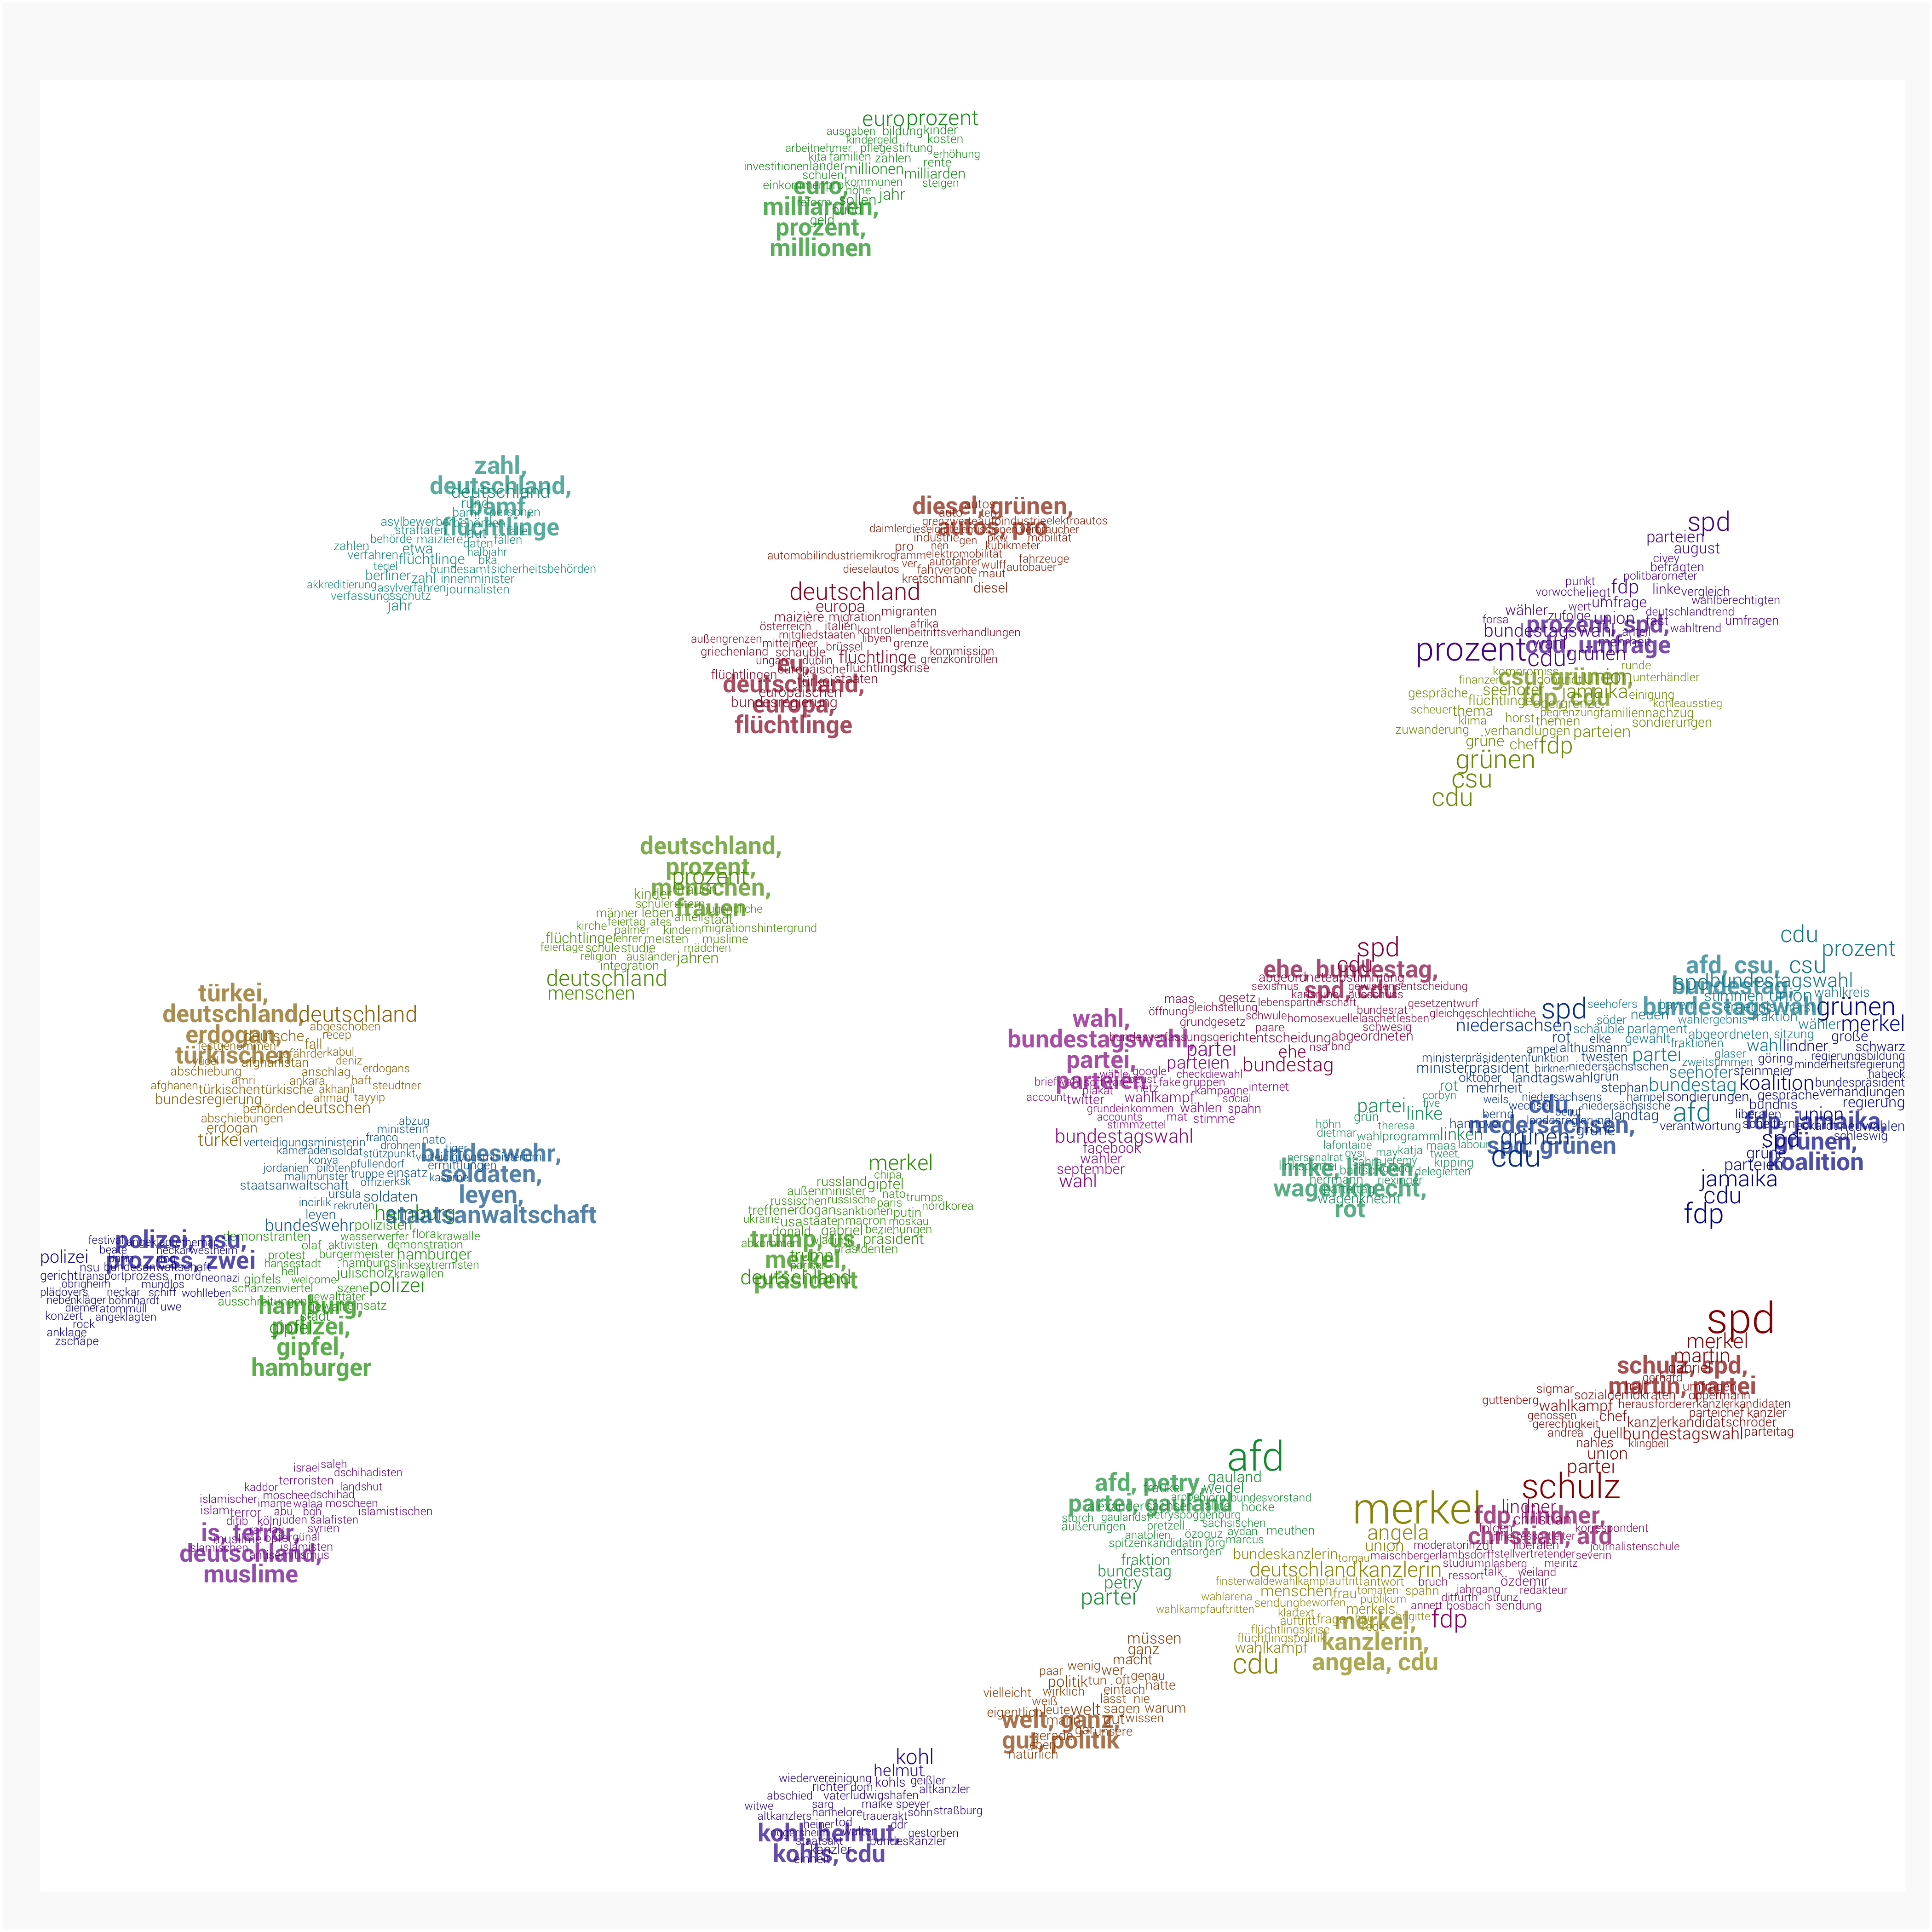
\includegraphics[width=\textwidth]{../figs/news-landscape-map.png}	
%	\label{fig_landscape}
%\end{figure}

%
%\begin{figure}[H]
%\centering
%	\caption{Sum of Facebook shares by topic}
%	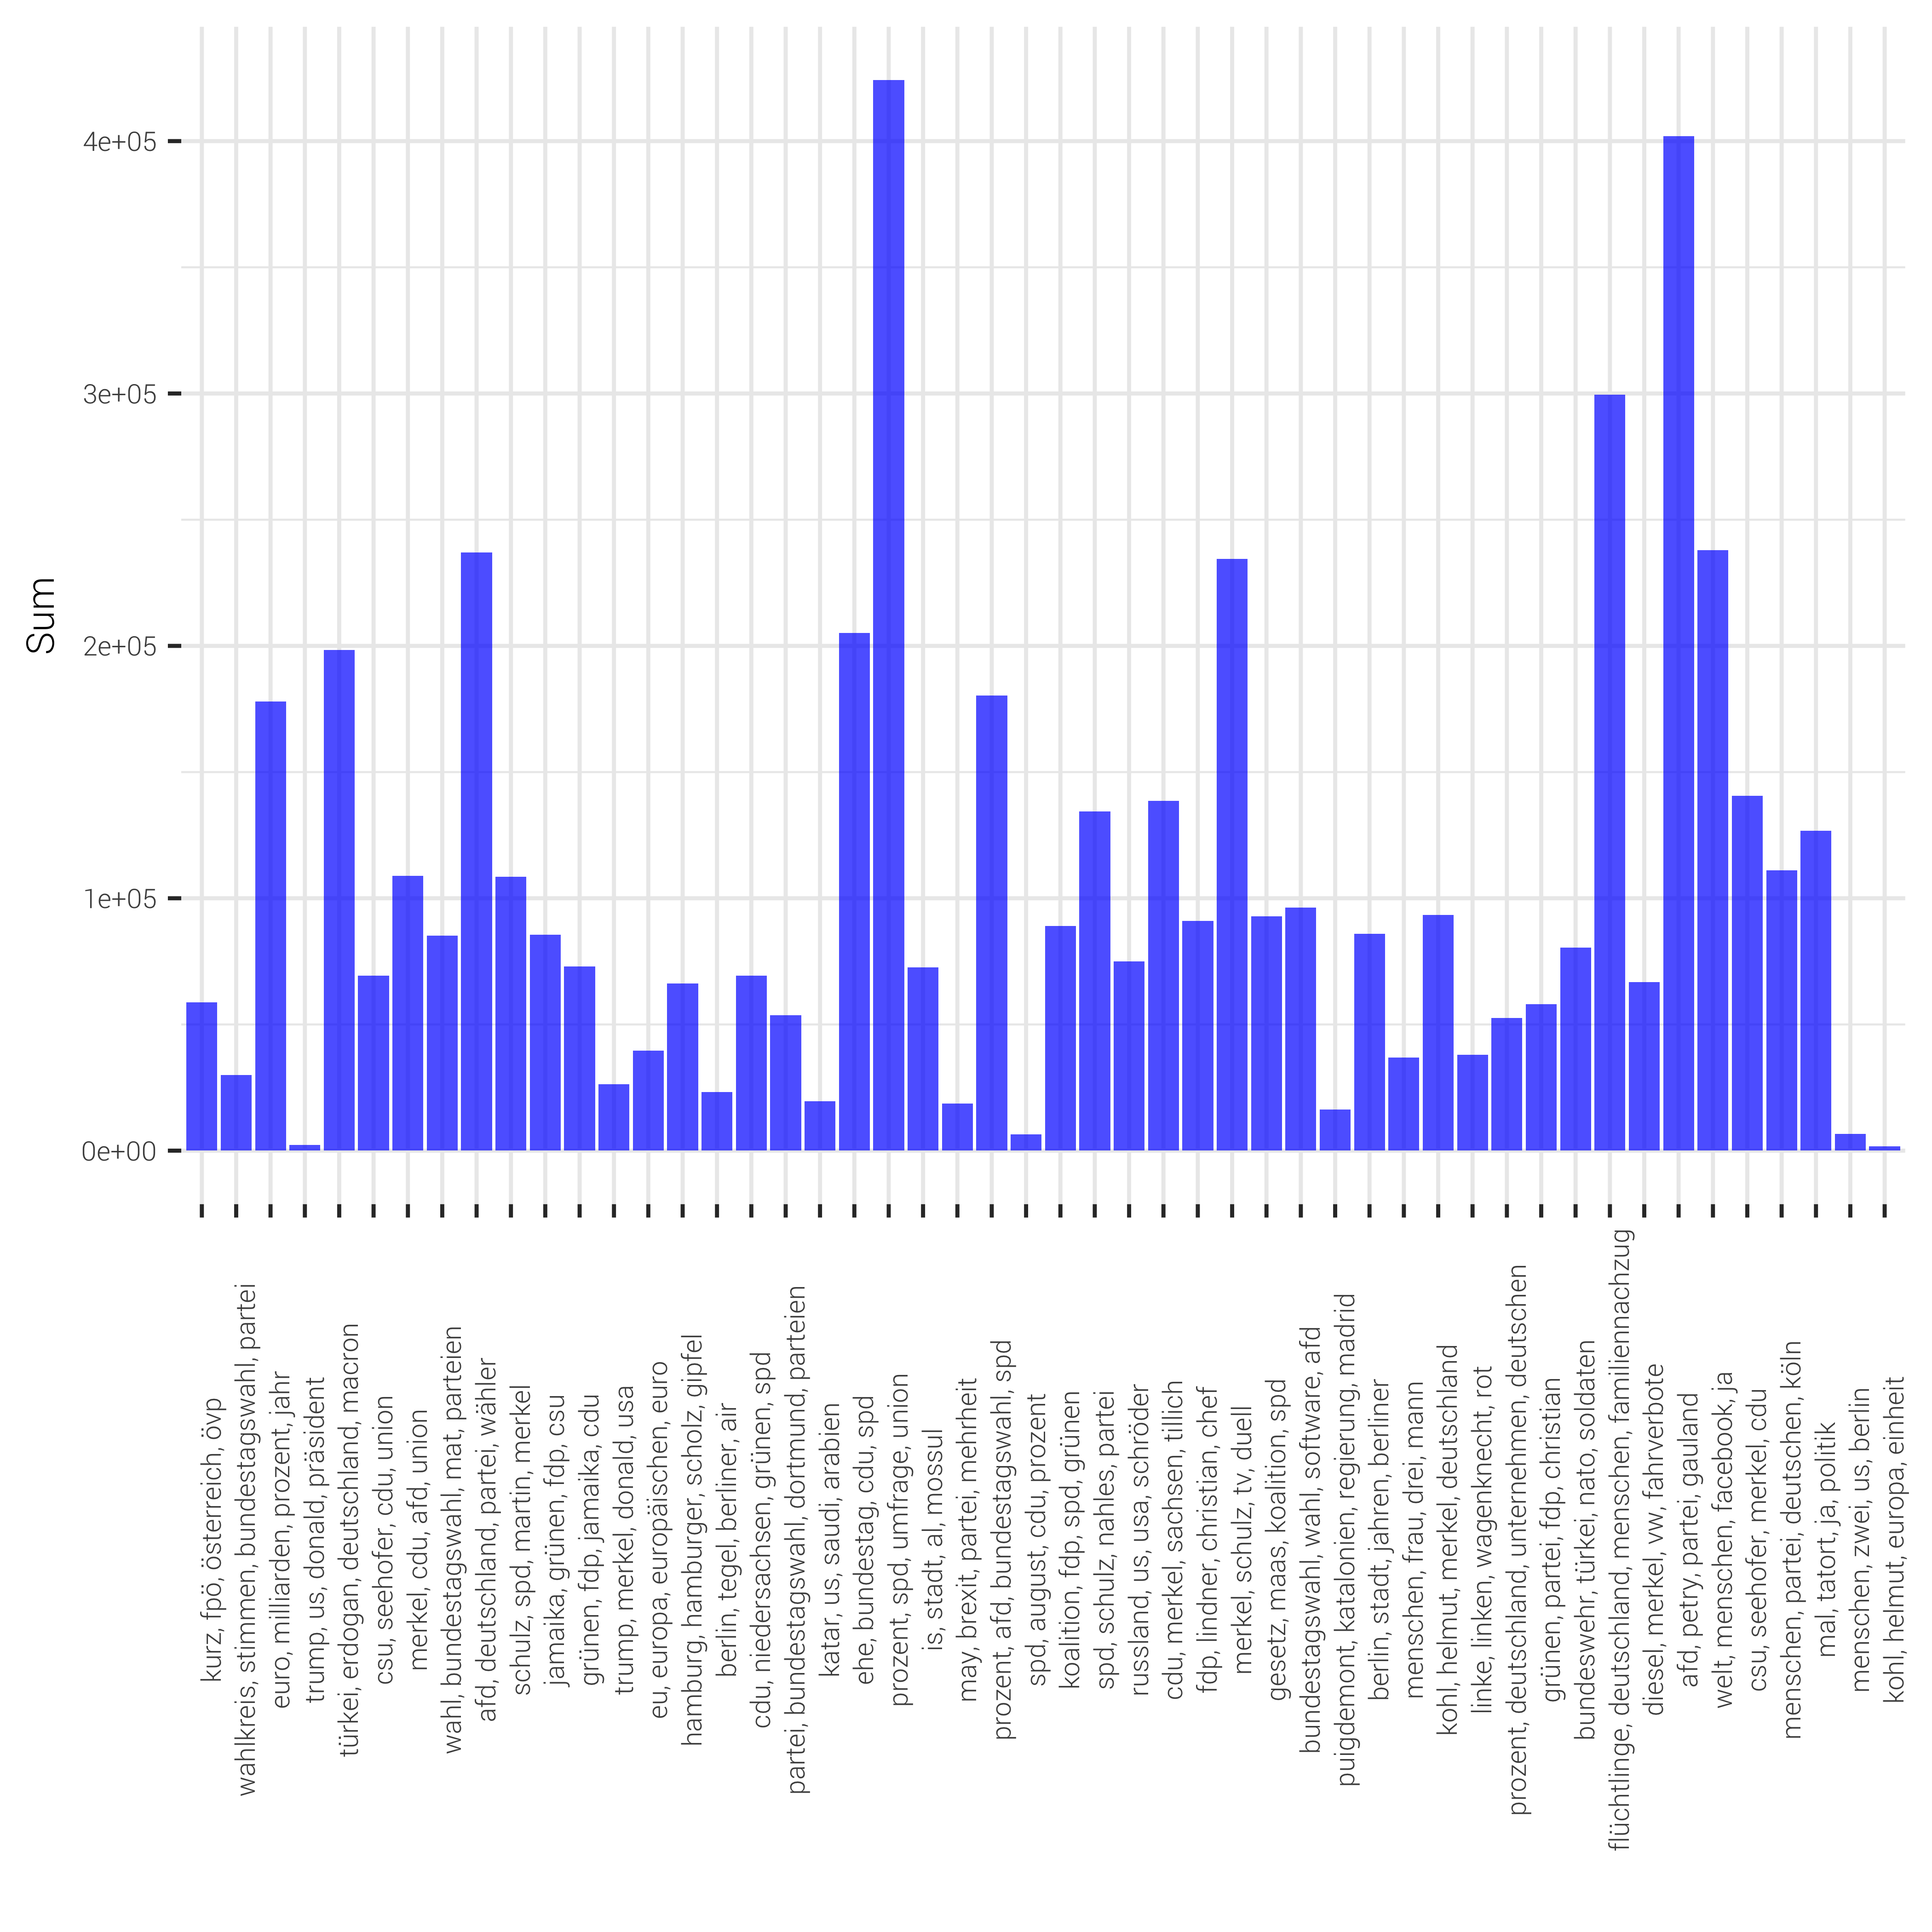
\includegraphics[width=\textwidth]{../figs/fb_shares_topics.png}	
%	\label{fig_fb_shares_topic}
%\end{figure}

\section{Regression}\label{ch_regression}

The examination of the topic probability distribution revealed that most documents are assigned a unique topic with high probability (65\% and higher), so that we can classify each document based on which topic has the highest probability. We keep only those documents, where the posterior probability of this topic is greater than 0.6 which left us with 6240 documents. 

The proportion of zeros in the independent variable (number of Facebook shares) is about 66\%. One way to model this type of situation is to assume that the data come from a mixture of two populations, one where the counts is always zero, and another where the count has a Poisson distribution with mean $\mu$. In this model zero counts can come from either population, while positive counts come only from the second one. 

The distribution of the outcome can then be modeled in terms of two parameters, $\pi$ the probability of 'always zero', and $\mu$, the mean number of publications for those not in the 'always zero' group. A natural way to introduce covariates is to model the logit of the probability $\pi$ of always zero and the log of the mean $\mu$ for those not in the always zero class.

The two-part model relaxes the assumption that the zeros (whether or not the article is shared) and positives (how often it is shared) come from the same data generating process. The zero-inflated model lets the zeros occur in two different ways: as a realization of the binary process (z=0) and as a realization of the count process when the binary variable z=1. 

If the process generating the zeros is $f_1(.)$ and the process generating the positive responses is $f_2(.)$ then the two-part hurdle model is defined by the following probabilities. 

\begin{align*}
	g(y)=\begin{cases}
		f_1(0) + 1(f_i(0))f_2(0) if y=0 \\
		(1-f_1(0))f_2(y) if y\geq 1
	\end{cases}
\end{align*}

The model for the zero versus positive responses is a binary model with the specified distribution, but we usually estimate it with the probit/logit model.

\end{document}
